\subsubsection{Fichiers}

\paragraph{Question 1} (Fichiers). Comme nous l'avons vu, l'allocation contiguë de fichiers conduit à une fragmentation du disque. Cette fragmentation est-elle interne ou externe ? Faites une analogie avec un point du chapitre "gestion de la mémoire".
\color{reponse}
\begin{itemize}
	\item La fragmentation externe est causée par l'allocation dynamique. Le problème est d'allouer des segments (c-à-d plusieurs blocs contigus) en minimisant le nombre de blocs (ou pages) inutilisés entre ces segments (c'est un peu comme Tetris) ;
	\item La fragmentation interne est causée par la taille fixe des blocs, et a lieu lorsqu'un bloc n'est pas entièrement utilisé.
\end{itemize}
\color{black}

\paragraph{Question 2} (Fichiers). Certains systèmes d'exploitation proposent un appel système \textbf{rename} pour donner un nouveau nom à un fichier. Existe-il une différence entre cette opération et celle qui consiste à faire une copie du fichier dans un nouveau fichier avec un nouveau nom et ensuite effacer le premier fichier ?
\color{reponse}
\begin{itemize}
	\item Oui. L'appel \textbf{rename} ne change pas l'heure de création ou l'heure de la dernière modification. En revanche, un nouveau fichier se voit attribuer l'heure actuelle comme heure de création et heure de la dernière modification. En outre, si le disque est plein, la copie peut échouer.
\end{itemize}
\color{black}



\paragraph{Question 3} (Fichiers). Considérons l'i-node de la Figure \ref{i-node}. S'il contient 10 adresses directes de 4 octets chacune et si tous les blocs sont de 1.024 octets, quelle est la taille maximale d'un fichier ?
\begin{figure}[p]
	\centering
	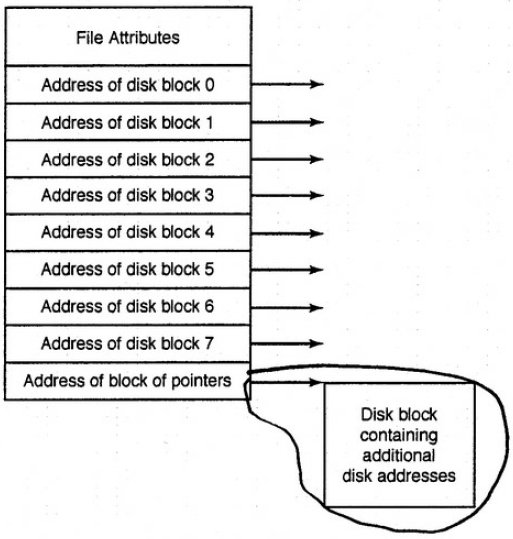
\includegraphics[scale=0.5]{images/i-node.png}
	\caption{\label{i-node} i-node}
\end{figure}
\color{reponse}
\begin{itemize}
	\item Le bloc indirect peut contenir 256 adresses disque. Avec kes 10 adresses disque directes, le fichier contient au maximum 266 blocs. Dans la mesure où chaque bloc a une taille de 1 Ko, la taille maximale d'un fichier est de 266 Ko.
\end{itemize}
\color{black}



\paragraph{Question 4} (Fichiers). On peut garder une trace de l'espace disque disponible à l'aide d'une liste de blocs libres ou d'une table de blocs libre (\textit{bitmap}). Les adresses disque nécessitent \textit{D} bits. Dans le cas d'un disque comprenant \textit{B}, dont \textit{F} sont libres, donnez la condition dans laquelle la liste de blocs libres utilise moins de place que la table de blocs libres. Pour \textit{D} égal à 16 octets, exprimez votre réponse en pourcentage de l'espace disque qui doit être libre. Faites une analogie avec un point du chapitre "gestion de la mémoire".
\color{reponse}
\begin{itemize}
	\item La table de blocs demande \textit{B} bits et la liste des blocs libres \textit{DF} bits. La liste de blocs libres nécessite moins de bits si \textit{DF < B} ou si \textit{F/B} est une fraction des blocs libres. Pour des adresses disque 16 bits, la liste des bits libres est plus courte si 6\% ou moins du disque sont libres.
\end{itemize}
\color{black}



\paragraph{Question 5} (Fichiers). Est-il raisonnable de défragmenter le disque ?
\color{reponse}
\begin{itemize}
	\item S'il est correctement effectué, oui. Pendant le compactage, chaque fichier doit être organisé pour que tous ses blocs soient consécutifs, afin d'accélérer l'accès. Les utilisateurs sont encouragés à l'exécuter périodiquement pour améliorer les performances du système. Compte tenu du temps nécessaire à cette tâche, une exécution par mois représente une bonne fréquence.
\end{itemize}
\color{black}



\paragraph{Question 6} (Fichiers). Le début d'une table de blocs libres juste après le formatage d'une partition disque ressemble à 1000.0000.0000.0000 (le premier bloc est utilisé par le répertoire racine). Le système recherche toujours les blocs libres à partir du bloc qui a le plus petit nombre ; ainsi après l'écriture du fichier \textit{A}, qui requiert 6 blocs, la table des blocs libres est de la forme : 1111.1110.0000.0000. Donnez la table après chacune des opération suivantes :
\begin{enumerate}
	\item Le fichier \textit{B} est écrit en utilisant 5 blocs.
	\item Le fichier \textit{A} est effacé.
	\item Le fichier \textit{C} est écrit en utilisant 8 blocs.
	\item Le fichier \textit{B} est effacé.
\end{enumerate}
\color{reponse}
\begin{itemize}
	\item Le début de la table de blocs ressemble à :
\end{itemize}
\begin{enumerate}
	\item 1111.1111.1111.0000
	\item 1000.0001.1111.0000
	\item 1111.1111.1111.1100
	\item 1111.1110.0000.1100
\end{enumerate}
\color{black}



\paragraph{Question 7} (Fichiers). Donnez un avantage des liens matériels par rapport aux liens symboliques et un avantage des liens symboliques vis-à-vis des liens matériels.
\color{reponse}
\begin{itemize}
	\item Les liens matériels ne demandent pas d'espace disque supplémentaire, mais simplement un compteur dans leur i-node pour suivre leur nombre, alors que les liens symboliques demandent de l'espace pour stocker le nom du fichier pointé. Les liens symboliques peuvent pointer vers des fichiers situés sur d'autres ordinateurs, voire sur internet, alors que les liens matériels sont limités aux fichiers de leur propre partition.
\end{itemize}
\color{black}



\paragraph{Question 8} (Fichiers). Nous avons étudié en détail les sauvegardes incrémentales. Sous Windows, il est facile de savoir quand sauvegarder un fichier, car chaque fichier possède un bit d'archivage. Mais ce bit est absent sous UNIX. De quelle manière les programmes de sauvegarde d'UNIX ont-ils connaissance des fichiers à sauvegarder ?
\color{reponse}
\begin{itemize}
	\item Ils doivent conserver l'heure de la dernière sauvegarde dans un fichier sur le disque. À chaque sauvegarde, on ajoute une entrée à ce fichier. Au moment de la sauvegarde, on lit le fichier et l'heure de la dernière entrée notée. Tout fichier modifié depuis cette heure est sauvegardé.
\end{itemize}
\color{black}